
% Works
% -----

\subsection{Conditional Operation and Inverse Sequences}

\begin{mydef}[$\works{x}$]
% Unsure if this relation should be in the algebra.
For a set of $k$ sequences
$\works{A_1,A_2,\ldots,A_k}$ means that 
$A_1,A_2,\ldots,A_k$ work at the same time, that is,
% intended interpretation:
\[\exists \FS: A_1\FS\neq\fsbroken \wedge \cdots \wedge A_k\FS\neq\fsbroken.\]
As the sequences form a set, their order is irrelevant.
% inference rules:
We also know that $\works{A} \Leftrightarrow A\nequiv \cbrk$. 
\end{mydef}

\begin{mydef}[$\worksc{x}{y}$]
For two sets of sequences, $\worksc{A_1,A_2,\ldots,A_k}{B_1,B_2,\ldots,B_l}$ means that 
all of $A_1,\ldots,A_k$ work where all of $B_1,\ldots,B_l$ work,
that is,
% intended interpretation:
\begin{align*}
\forall \FS:{}& 
B_1\FS\neq\fsbroken \wedge \cdots \wedge B_k\FS\neq\fsbroken\\
&\Rightarrow\\
&A_1\FS\neq\fsbroken \wedge \cdots \wedge A_l\FS\neq\fsbroken.
\end{align*}
As above, the order of the sequences in the sets is not relevant.
\end{mydef}

\begin{mydef}[Sets of sequences]
As we will frequently refer to sets of fequences,
we will use calligraphic letters (e.g. $\seqset{A, B, C}$ and $\seqset{S}$)
to denote such sets for brevity.
We will use $A\cc\seqset{B}$ to denote the set of sequences $\{A\cc B|B\in\seqset{B}\}$.
\end{mydef}

It is easy to see that the following corollaries are true:

% An inference rule in the algebra
% $\worksc{X}{X}$ is always true for any set of sequences $X$,

% \begin{mycor}
% % An inference rule in the algebra
% $B\eqext A \Rightarrow \worksc{A}{B}$.
% \end{mycor}

\begin{mycor}\label{worksextpostfix}
% An inference rule in the algebra
$\forall A,S: \worksc{A}{A\cc S}$, that is, if a sequence works, its initial segment also works.
\end{mycor}

\begin{mycor}\label{workschained}
% An inference rule in the algebra
$\workssign$ can be chained:
if $\seqset{A'}\subset\seqset{A}$, then
$ \worksc{\seqset{C}}{\seqset{A'}} \wedge \worksc{\seqset{A}}{\seqset{B}} \Rightarrow \worksc{\seqset{A}\cup\seqset{C}}{\seqset{B}}$.
\end{mycor}

We also prove the following lemmas.

\begin{myax}\label{combine_independent_commands}
The combination of independent commands works wherever the original commands work:
\[ \cxynv\indep \czwmv \Rightarrow \worksc{\cxynv\cc \czwmv}{\cxynv, \czwmv}. \]
% \begin{align*}
% \forall\FS:{}&\cxynv\indep \czwmv \\
% &\quad\wedge \cxynv\aFS\neq\fsbroken \\
% &\quad\wedge \czwmv\aFS\neq\fsbroken \\
% &\Rightarrow \cxynv\cc \czwmv\aFS\neq\fsbroken.
% \end{align*}
\end{myax}
\begin{proof}
We name this proposition a \namecref{combine_independent_commands} 
because to prove it, we must reach back to our filesystem model.
We proceed in an indirect way and
assume that there is a filesystem $\FS$ for which
$\cxynv\aFS\neq\fsbroken$ and $\czwmv\aFS\neq\fsbroken$, but
$\cxynv\cc \czwmv\aFS=\fsbroken$.
We know $\cxynv\aFS\neq\fsbroken$ so it must be applying 
$\czwmv$ that breaks it.
Applying a command can only result in a broken filesystem in three cases.
First, if the filesystem was already broken, which cannot be the case here.
Second, if the input type does not match the filesystem,
but we know $\FS(m)\in\setvx{W}$ and so
$(\cxynv\aFS)(m)\in\setvx{W}$ as based on \cref{incomparable_is_independent}, $n\neq m$.
Third, if the new filesystem violates the tree property.
This again cannot be the case because we also know that $n\unrel m$
and the tree property only depends on the types of the parent and children of $m$,
which therefore cannot be changed by $\cxynv$.
\end{proof}

This result can be extended to sequences:

\begin{mylem}\label{combine_independent_sequences}
The combination of independent sequences works wherever the original sequences work:
\[ S\indep T \Rightarrow \worksc{S\cc T}{S,T}. \]
\end{mylem}
\begin{proof}
Assume that there is a filesystem $\FS$ so that
$S\aFS\neq\fsbroken$ and $T\aFS\neq\fsbroken$, but
$(S\cc T)\FS=\fsbroken$.

From \cref{incomparable_is_independent,ax_separate_commute} we know that
the commands in $S$ and $T$ pairwise commute, and so any sequence
that contains the commands from $S$ and $T$ and preserve their original partial order
is equivalent to $S\cc T$ on all filesystems.

Let the command that breaks $\FS$ in $T$ when applying $S\cc T$ be $t$
so that $T=T_0\cc t\cc T_1$.
It is still true that $(T_0 \cc t)\FS\neq\fsbroken$,
and by definition $(S\cc T_0)\FS\neq\fsbroken$,
but $(S\cc T_0\cc t)\FS=\fsbroken$.
Also, from above we know that $S\cc T_0\equiv T_0\cc S$
and so $(T_0 \cc S)\FS\neq\fsbroken$.

If we denote the first command in $S$ with $s_1$,
this means that $(T_0 \cc s_1)\FS\neq\fsbroken$,
which we can combine with $(T_0 \cc t)\FS\neq\fsbroken$, $t\indep s_1$ and
\cref{combine_independent_commands}
(using $T_0\FS$ as the reference filesystem)
to arrive at $(T_0 \cc s_1\cc t)\FS\neq\fsbroken$.

We can repeat this step for $s_2$, the next command in $S$,
and from 
$(T_0 \cc s_1\cc t)\FS\neq\fsbroken$
and
$(T_0 \cc s_1\cc s_2)\FS\neq\fsbroken$
arrive at
$(T_0 \cc s_1\cc s_2\cc t)\FS\neq\fsbroken$.
This can be repeated until $S$ is exhausted and we get
$(T_0 \cc S\cc t)\FS\neq\fsbroken$, which is a contradiction.
\end{proof}

We also prove the following:

\begin{mylem}\label{worksinputmatch}
If $A$ and $B$ are minimal sequences, $\works{A,B}$,
and there are commands on node $n$ in both $A$ ($\cxynv\in A$) and $B$ ($\czwnv\in B$),
then the input types of these commands must match ($X=Z$).
\end{mylem}
\begin{proof}
This result is similar to \cref{equiv_simple_same_commands} and
is easily shown using an indirect proof: if $X\neq Z$, then there is no filesystem that
either $\cxynv$ or $\czwnv$ would not break, 
and consequently $A$ and $B$ cannot work on the same filesystem.
\end{proof}


\bigskip

%% TODO https://en.wikipedia.org/wiki/Equivalence_class

\noindent
We know that whether commands break a filesystem depends solely on their input and output
types and the node, but not their actual output value.
To represent this, we introduce an equivalence relation between filesystems, commands
and sequences of commands.
\begin{mydef}[Equivalence by type: $\typeeq$]
$ $ % otherwise first list element starts on same line
\begin{itemize}
\item For two filesystems we write $\FS\typeeq\GS$ iff they are both broken, or they share the same nodes,
and at all nodes the types of their values are the same.
\item For two commands we write $\alpha\typeeq\beta$ iff their input and output types,
and the node they operate on are the same.
For example, $\cbfaa{n}{f_1}\typeeq\cbfaa{n}{f_2}$.
\item For two sequences of commands we write $A\typeeq B$ iff they contain the same number of commands,
and pairwise the commands $\alpha\in A$ and $\beta\in B$ at the same indices are equivalent by type ($\alpha\typeeq\beta$).
\end{itemize}
\end{mydef}

In other words, two type-equivalent objects can only differ in the value they contain,
but as $|\setb|=|\setd|=1$, this is only possible at values of the type $\ccharf$.
We select an arbitrary file value $\fil\in\setf$, and choose a representative
of each $\typeeq$-equivalence class where all (if any) values of the type $\ccharf$ is $\fil$.
For example, in the case of commands, the representative of $[\cbfaa{n}{f}]_\typeeq$ is $\cbfaa{n}{\fil}$.

\begin{mydef}[$\T$]
We use $\T$ and write $x\T$ to denote the canonical mapping of 
filesystems, commands and sequences to the
representatives of their $\typeeq$-equivalence class.
$\T$ is also extended to sets of sequences,
where $\seqset{A}\T = \{S\T | S\in\seqset{A}\}$.
\end{mydef}

For example, $\cbfaa{n}{f}\T = \cbfaa{n}{\fil}$,
and for the sequence $S=\alpha\cc\beta$, $S\T=\alpha\T\cc\beta\T$.
In other words, $\T$ maps our system of filesystems and commands
into a system where $|\setf|$ is also $1$.

\begin{mycor}
For any filesystem $\FS$ and command $\alpha$, 
$\alpha\T(\FS\T) = (\alpha\aFS)\T$.
\end{mycor}

% It is easy to see that 
% $A\equiv B \Rightarrow A\T\equiv B\T$ 
% and
% $A\eqext B \Rightarrow A\T\eqext B\T$,
% but the reverse is not true as 
% $A\T$ and $B\T$ will have the same effect on all filesystems
% if $A$ and $B$ differ only in some of the values in their commands,
% whereas clearly $A\nequiv B$.

As whether a sequence of commands breaks a filesystem does not depend on the output values
of the commands, only the input and output types, we know that
\begin{mycor}
\begin{gather*}
\works{\seqset{A}} \Leftrightarrow \works{\seqset{A}\T} \\
\worksc{\seqset{A}}{\seqset{B}} \Leftrightarrow \worksc{\seqset{A}\T}{\seqset{B}\T}.
\end{gather*}
\end{mycor}


We are now ready to define the inverse of representative commands $\alpha\T$
which allows us to move parts of sequences between the
condition and consequence parts of $\workssign$.
This is based on the following observation.

\begin{mylem}
Representative functions $\alpha\T$ are injections over representative filesystems ($\FS\T$)
except for the cases where they break a filesystem, that is,
\[ \forall\FS,\GS,\alpha: \FS\T\neq\GS\T \wedge \alpha\T(\FS\T)\neq\fsbroken \Longrightarrow \alpha\T(\FS\T) \neq \alpha\T(\GS\T). \]
\end{mylem}
\begin{proof}
This is trivial if $\GS\T=\fsbroken$, so we assume it is not so.
If $\FS\T$ and $\GS\T$ have different values at any node apart from $n$, then this difference remains
even after applying the command to $\FS\T$. The only remaining case therefore is where they have the same values
at all nodes except $n$.
We know that a representative filesystem can only have values from the set $\rvalueset$.
As $\alpha\T(\FS\T)\neq\fsbroken$, $\FS\T(n)$ must be the value that matches the input type of $\alpha\T$.
We know that $\GS\T(n)\neq\FS\T(n)$, and therefore $\GS\T(n)$ must have a different type,
which implies $\alpha\T(\GS\T)=\fsbroken$ as it cannot match the input type of $\alpha\T$,
and again we have $\alpha\T(\FS\T) \neq \alpha\T(\GS\T)$.
\end{proof}

\begin{mydef}[Inverse commands and sequences]
If we regard the representative command $\alpha\T$ a function whose
domain is the subset of representative filesystems $\{\FS\T | \alpha\aFS\neq\fsbroken\}$,
then we can define the inverse of $\alpha\T$
for which we write $\alpha\T^{-1}$.
We write ${S\T}^{-1}$ for the inverse of the sequence $S\T$, which consists of the inverses of the commands in $S\T$
in reverse order.
\end{mydef}


From the definitions we can clearly see that
\begin{mycor}\label{negneg_is_typeeq} %% TODO Don't use!
$\forall S, \FS: (S^{-1})^{-1}\aFS\typeeq S\aFS$.
\end{mycor}

\begin{mylem}\label{r_invmove}
A common initial segment of a set of sequences can be moved to the other side of $\workssign$ by inverting it:
\begin{gather*}
\worksc{B\cc \seqset{A}}{\seqset{C}} \Rightarrow \worksc{\seqset{A}}{B^{-1}\cc \seqset{C}} \\
\worksc{\seqset{A}}{B\cc \seqset{C}} \Rightarrow \worksc{B^{-1}\cc \seqset{A}}{\seqset{C}}
\end{gather*}
\end{mylem}
\begin{proof}

%% TODO see lemma above

This is based on the fact that in our model, unless they break a filesystem,
commands leave the type of the filesystem value unchanged 
or change one type into another, but never merge types.
That is,
sequences---as functions mapping filesystems to filesystems---are
essentially bijections over type-equality ($\typeeq$)
with the only ``sink'' being $\fsbroken$:
\begin{align*}
\forall S,\FS,\GS:{}&S\aFS\neq\fsbroken \Rightarrow \\
&(S\aFS\ntypeeq S\aGS \Longleftrightarrow \FS\ntypeeq \GS).
\end{align*}

For the proposition
\[ \worksc{B\cc \seqset{A}}{\seqset{C}} \Rightarrow \worksc{\seqset{A}}{B^{-1}\cc \seqset{C}} \]
the rest of the proof is illustrated by \cref{fig_invmove}
where $\textrm{Dom}(x)$, the domain of $x$, represents the set of filesystems
the sequence $x$ does not break, or neither of the sequences in the set $x$ breaks.

\begin{figure}[htb]
\begin{center}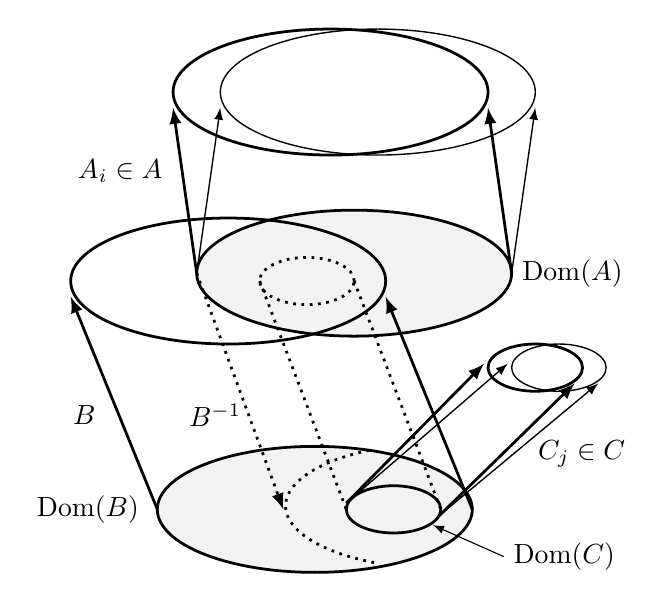
\begin{tikzpicture}
[line width=1pt]
\node at  (1.6+2, 0.1) [right] {$\textrm{Dom}(\seqset{A})$};
\draw[fill=black!5]     (1.6, 0.1) ellipse (2cm and 0.8cm); %% Dom A
\draw                   (1.3, 2.4) ellipse (2cm and 0.8cm); %% Img A1
\draw[line width=0.5pt] (1.9, 2.4) ellipse (2cm and 0.8cm); %% Img A2
\draw[-latex]                  (1.6+2, 0.1)--(1.3+2, 2.4-.2); %% A1 right
\draw[-latex]                  (1.6-2, 0.1)--(1.3-2, 2.4-.2); %% A1 left
\draw[-latex,line width=0.5pt] (1.6+2, 0.1)--(1.9+2, 2.4-.2); %% A2 right
\draw[-latex,line width=0.5pt] (1.6-2, 0.1)--(1.9-2, 2.4-.2); %% A2 left
\node at  (1.4-2-.1, 1.4) [left] {$A_i\in\seqset{A}$};
%%
\node at (1.1-2-.1, -2.9) [left] {$\textrm{Dom}(B)$};
\draw[fill=black!5] (1.1, -2.9) ellipse (2cm and 0.8cm); %% Dom B
\draw               (0  ,  0)   ellipse (2cm and 0.8cm); %% Img B
\draw[-latex] (1.1+2, -2.9)--(0+2, 0-.2); %% B right
\draw[-latex] (1.1-2, -2.9)--(0-2, 0-.2); %% B left
\node at  (0.55-2-.1, -1.7) [left] {$B$};
\draw[-latex,dotted] (1.6-2, 0.1)--(0.7, -2.9); %% B-1
\node at (0.3, -1.7) [left] {$B^{-1}$};
\draw[dotted] (1.79, -2.15) arc(118:244: 2cm and 0.8cm); %% Arc
\draw[dotted] (1, 0) ellipse (0.6cm and 0.3cm); %% Dotted S
\draw         (2.1, -2.9) ellipse (0.6cm and 0.3cm); %% Dom S
\draw[dotted] (1-0.6, 0)--(2.1-0.6, -2.9); %% B-1
\draw[dotted] (1+0.6, 0)--(2.1+0.6, -2.9); %% B-1
\draw                     (3.9, -1.1) ellipse (0.6cm and 0.3cm); %% Img S1
\draw[line width=0.5pt]   (4.2, -1.1) ellipse (0.6cm and 0.3cm); %% Img S2
\draw[-latex]                  (2.1-0.6, -2.9+.08)    --(3.9-0.6-.05, -1.1+.05); %% Left S1
\draw[-latex]                  (2.1+0.6-.02, -2.9-.08)--(3.9+0.6-.1, -1.1-.2); %% Right S1
\draw[-latex,line width=0.5pt] (2.1-0.6, -2.9+.08)    --(4.2-0.6-.05, -1.1+.05); %% Left S2
\draw[-latex,line width=0.5pt] (2.1+0.6-.02, -2.9-.08)--(4.2+0.6-.1, -1.1-.2); %% Right S2
\node at  (3.8,-2.2) [right] {$C_j\in\seqset{C}$};
\draw[-latex,thin] (3.5, -3.5) node[right]{$\mathrm{Dom}(\seqset{C})$} -- (2.1+0.5, -2.9-0.2);
\end{tikzpicture}\end{center}

\caption{Proof of \cref{r_invmove}}\label{fig_invmove}
\end{figure}

We see that the set of filesystems the sequences in $\seqset{A}$ do not break intersect with the range of $B$.
As $B$ is a bijection between its domain and range, we can use $B^{-1}$ to map this intersection back
onto the domain of $B$.
As $\worksc{B\cc \seqset{A}}{\seqset{C}}$ the domain of $\seqset{C}$ must be a subset of this
projected intersection.
If so, then we can use $B$ to map the domain of $\seqset{C}$, which yields the domain of $B^{-1}\cc \seqset{C}$.
As it is also a part of the domain of $A$, we get $\worksc{\seqset{A}}{B^{-1}\cc \seqset{C}}$.

The second part of the lemma can be proven in a similar way.
\end{proof}


\begin{mylem}\label{indep_prefix_combine}
The combination of sequences with a common head and independent tails 
continues to work under the same conditions:
\[ \worksc{A\cc B}{\seqset{S}} \wedge \worksc{A\cc C}{\seqset{S}} \wedge B\indep C \Rightarrow \worksc{A\cc B\cc C}{\seqset{S}} \]
\end{mylem}
\begin{proof}
Based on \cref{r_invmove} we know
$\worksc{B}{A^{-1}\cc \seqset{S}}$ and $\worksc{C}{A^{-1}\cc \seqset{S}}$,
and from \cref{combine_independent_sequences} we know
$\worksc{B\cc C}{B,C}$.
Combining these using \cref{workschained}
we get
$\worksc{B\cc C}{A^{-1}\cc \seqset{S}}$. 
Finally, applying the second line of \cref{r_invmove} yields
$\worksc{(A^{-1})^{-1}\cc B\cc C}{\seqset{S}}$, which proves our lemma 
as $\forall\FS: (A^{-1})^{-1}\aFS\typeeq A\aFS$ (\cref{negneg_is_typeeq}).
\end{proof}
